%
%  Vincent Yannello
%
\documentclass[12pt,fullpage]{article}
\usepackage{fullpage}
\usepackage{psfrag}                                          % LaTeX graphics tool
\usepackage{pslatex}                                         % avoids the default cmr font
\usepackage{graphicx}                                        % graphics package 
\usepackage{epsfig}                                          % figures
\usepackage{hyperref}
\usepackage{color}

\begin{document}

\noindent
{\bf Error distribution} (from \color{blue}\url{http://www.math.wm.edu/~leemis/chart/UDR/UDR.html}\color{black})

\noindent
The shorthand $X \sim {\rm error}(a, b, c)$ is used to indicate that the
random variable $X$ has the error distribution with location parameter $a$, scale parameter $b$, and shape parameter $c$.
An error random variable $X$ with parameters $a$, $b$, and $c$ has probability density function 
$$
f(x) = \frac{{e^{\left( -{\left| x-a \right|/b} \right) ^{2/c}/2}}}{b({2}^{c/2+1}) \Gamma  \left( c/2+1 \right)} \qquad \qquad -\infty < x < \infty
$$
for all real values $a$ and for $ b > 0$, $c > 0$.
The probability density function with three different parameterizations is illustrated below.
{\begin{figure}[h!]
\begin{center}
\psfrag{lab1}{$a = -1,\  b = 1,\  c = 0.25$}
\psfrag{lab2}{$a = -1,\  b = 0.5,\  c = 1$}
\psfrag{lab3}{$a = 0,\  b = 1,\  c = 2$}
\psfrag{labx}{$x$}
\psfrag{labf}{$f(x)$}
\includegraphics[width=3.2in]{ErrorPlot.ps}
\end{center}
\end{figure}}\\
The cumulative distribution function on the support of $X$ is
$$
F(x) = P(X \le x) = \int_{-\infty}^x\frac{{e^{\left( -\left| t-a \right|/b \right) 
^{2/c}/2}}}{b({2}^{c/2+1}) \Gamma  \left( c/2+1 \right)}dt \qquad \qquad -\infty < x < \infty.
$$
The survivor function, hazard function, inverse distribution function, moment generating function, 
and characteristic functions are all mathematically intractable.
The population median and mode of $X$ occurs at $x = a$.
The population mean, variance, skewness, and kurtosis of $X$ are 
$$
E[X] = a \qquad \qquad V[X] = \frac{2 ^ c b ^ 2 \Gamma(3c / 2)}{\Gamma(c/2)}.
$$
$$
E\left[ \left( \frac{X - \mu}{\sigma} \right) ^ 3 \right] = 0 \qquad \qquad
E\left[ \left( \frac{X - \mu}{\sigma} \right) ^ 4 \right] = \frac{\Gamma(5c / 2) \Gamma(c / 2)}{(\Gamma(3c/2)) ^ 2}.
$$
%
%  Moments taken from page 86 the 4th edition of Forbes, Evans, Hastings, Peacock
%

\vspace{0.1in}
\newpage
\noindent
{\bf APPL verification:}
The APPL statements
%                                  X := ErrorRV(a, b, c);
\begin{verbatim}
assume(b > 0);
assume(c > 0);
X := [[x -> exp((-abs(x - a) / b) ^ (2 / c) / 2) / (b * (2 ^ (c / 2 + 1)) *
       GAMMA(c / 2 + 1))], [-infinity, infinity], ["Continuous", "PDF"]];
CDF(X);
SF(X);
HF(X);
CHF(X);
Mean(X);
Variance(X);
Skewness(X);
Kurtosis(X);
MGF(X);
\end{verbatim}
fail due to integration problems.
%The Maple code
%\begin{verbatim}
%assume(b > 0);
%assume(c > 0);
%area := int(exp((-abs(x - a) / b) ^ (2 / c) / 2) / (b * (2 ^ (c / 2 + 1)) *
%            GAMMA(c / 2 + 1)), x = -infinity .. a) +
%        int(exp((-abs(x - a) / b) ^ (2 / c) / 2) / (b * (2 ^ (c / 2 + 1)) *
%            GAMMA(c / 2 + 1)), x = a .. infinity);
%\end{verbatim}
%These fail except when a = 0 and c = 2.
\end{document}
